\section{Synthesis: comparing the DiVaS and ALoVaS methods}
In this section we compare the DiVaS and ALoVaS models. While both methods seem relatively similar, both methods performing variable selection on Bayesian decision trees, there are fundamental practical and theoretical differences between the two methods. 

\subsection{Theoretical differences and a simulation study}

One of the most apparent theoretical differences between the DiVaS and ALoVaS models is the way the two models handle the correlation between covariate selection probabilities. One of the properties of the Dirichlet distribution is that $Corr(p_i,p_j) < 0$ for $i\neq j$. Thus if the prior puts zero probability on non-negative covariate selection probability correlations then the posterior will also place zero probability on these non-negative correlations. This section elucidates the differences between the two methods and compares the similarities. 


%%%% Start of graphic

%\PreviewEnvironment{tikzpicture}
%\setlength\PreviewBorder{5pt}%
\begin{figure}[H]
\begin{center}
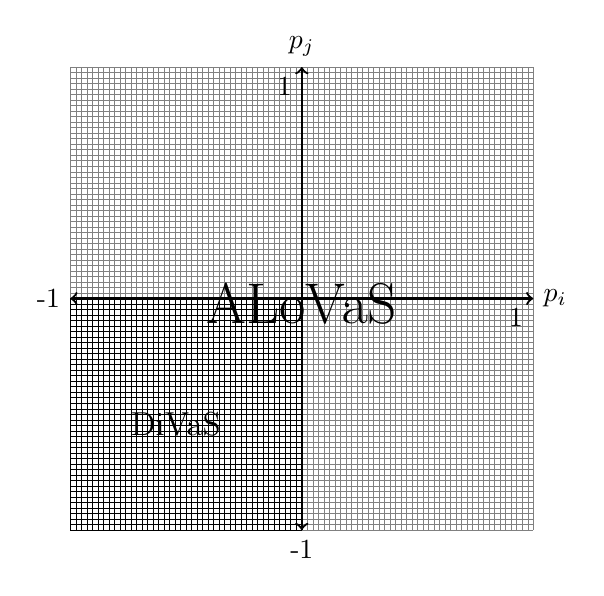
\begin{tikzpicture}[scale=.35]%\footnotesize
% grid
 
  %\draw[step=0.1cm,gray,very thin] (\xone,\yone) grid (8,8);
  \draw[step=0.2cm,gray,very thin] (-.4,-.4) grid (16.4,16.4);
  \draw[step=0.2cm,black,very thin] (-.4,-.4) grid (8,8);

% ticks
  \foreach \x/\xtext in { 8/\frac{1}{2}, 16/1}
  \draw[gray, very thin,xshift=\x cm] (0,.3) -- (0,-0.3) node[below] {};
  \draw[gray, very thin] (0,-0.3) node[below] {};
  \foreach \y/\ytext in {8/\frac{1}{2},16/1}
    \draw[gray, very thin, yshift=\y cm] (.3,0) -- (0,0)
    node[left] {};

% origin
 \draw[gray] (0,0) node[anchor=north east] {};

% labels 
\draw (3.43,3.43) node[circle]{\large{DiVaS}} circle (0cm);
\draw[thick] (8,7.8) node[]{\huge{ALoVaS}} circle (0cm);

% axes
  \draw[black,thick,<->] (-.4, 8) -- (16.4, 8) node[right] {$p_i$};
  \draw[black,thick,<->] (8, -.4) -- (8, 16.4) node[above] {$p_j$};
   \draw[black,thick] (16.4, 8) node[below left] {1};
  \draw[black,thick] (-.4, 8) node[left] {-1};
   \draw[black,thick] (8,16.4) node[below left] {1};
  \draw[black,thick] (8, -.4) node[below] {-1};

%  \draw[black,thick,<->] node[above] {$p_j$};
\end{tikzpicture}
\end{center}
\end{figure}

%%%% End of graphic


One might be tempted to conclude that this is a element of minut\ae\ that has no practical consequence but consider a linear model data generating process that contains an interaction between two variables, $x_1$ and $x_2$

\begin{equation}\label{eqn:interaction_model}
y_i = \beta x_1x_2 + \epsilon_i,
\end{equation}  
where $\epsilon_i \sim N(0, \sigma^2$). In this case the coefficient $\beta$ controls the degree of curvature in the $x_1, x_2$ space. The positive covariate selection probability results from using a constant function in each terminal node to approximate a curved two dimensional surface. The constant function requires alternating splits between $x_1$ and $x_2$ to approximate the curving of the $x_1$, $x_2$ space. Thus, we see that there are really two important pieces to the model specification when fitting decision trees: specifying a tree model and specifying a terminal node model. Misspecification of 1 can lead to errors in the other indicating that the two are also not independent.

A nice property of the ALoVaS method is that the if $p_i$, $p_j$ be the two covariate selection probabilities, then if these $p_i$, $p_j$ have a logistic normal density the covariance between the two densities is 

\begin{equation}\label{eqn:cov_aln}
Cov(log(p_j / p_k), log(p_l / p_m) ) = \sigma_{jl} + \sigma_{km} - \sigma_{jm} - \sigma_{kl},
\end{equation}
where $\sigma_{ij}$ is the covariance parameter for the normal random variable before the application of the ALT. Clearly the four $\sigma_{ij} \geq 0$ in Equation \ref{eqn:cov_aln} so that the covariance could be positive or negative.  

At this point it is worth noting that the idea of an automatic interaction detector was first proposed in the CHAID method \cite{kass1975significance}. The CHAID method claims to automatically detect interactions, yet popular documents \cite{ville2006decision} claim that CHAID and other decision tree methods cannot actually perform automatic interaction detection. The validity of this claim is not the point of this paragraph but it should be clear to the reader how one could visually inspect a fitted tree and determine if interaction is plausible. Moreover, with the ALoVaS method automatic interaction detection is plausible, by comparing the sampled values of $Cov(log(p_j/p_k), log(p_l/p_m) )$, or equivalently $Corr(p_i, p_j)$, against the point zero one gets an indication of the degree of interaction. Additionally, we cannot determine if the interaction is positive or negative, only that an interaction is present. If there was a desire to determine the sign of the interaction then the analyst would need to provide estimates of the parameters in Equation \ref{eqn:cov_aln} or alternately, we might estimate directly $Corr(p_i, p_j)$ with the Bayesian approach we take in the ALoVaS method, either approach is feasible. 

We now present a small simulation study. We sampled data according to the model describing in Equation \ref{eqn:interaction_model}. We simulated $n=500$ observations from this model for a training and another for a test, or hold-out data set. We simulated data under the model with $\beta \in \{5, -5\}$. The trees fitted under a greedy optimization for the two interaction scenarios are shown in Figure \ref{fig:interaction_trees}. 

\begin{figure}
\begin{center} 
\begin{tabular}{cc}
%  \num\putindeepbox[2pt]{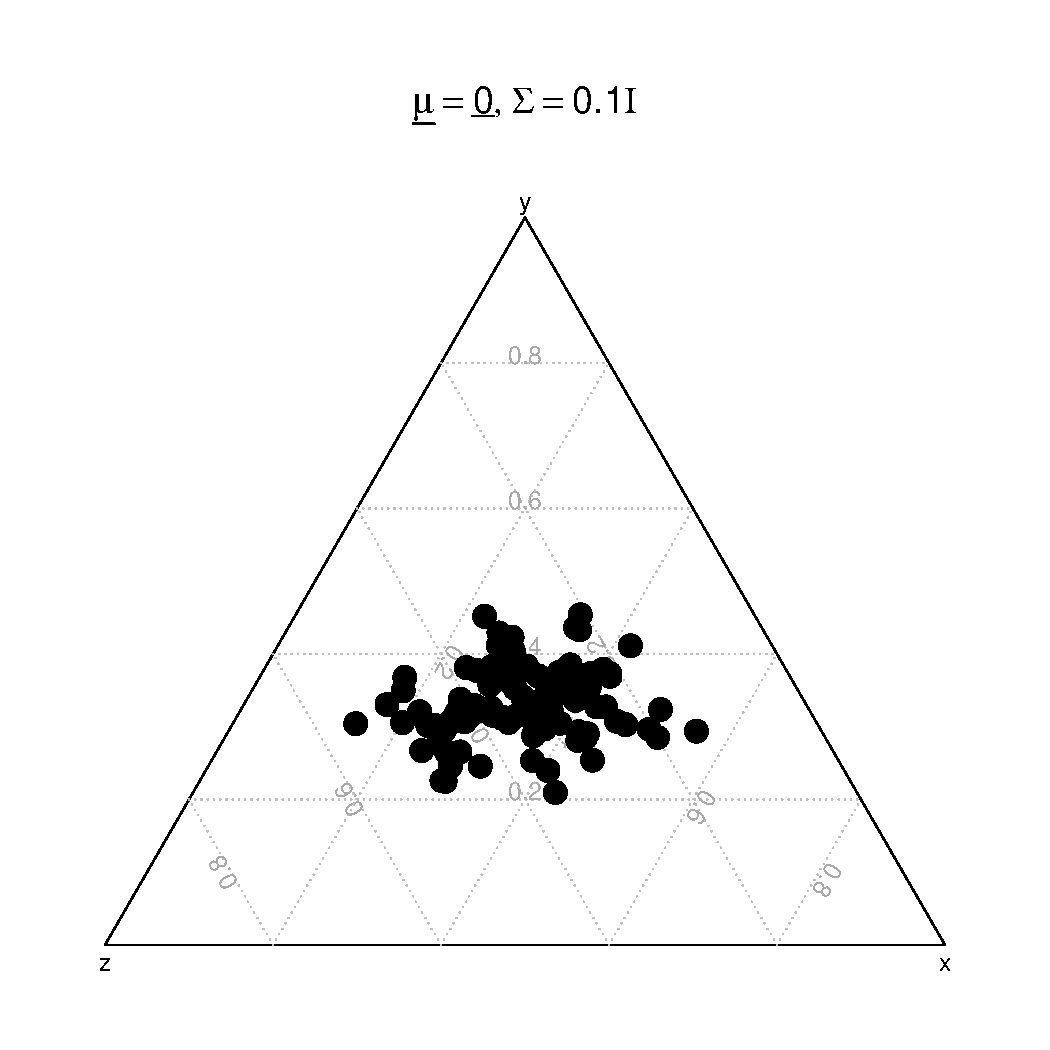
\includegraphics[scale=0.25]{figures/mu0_0_bw.pdf}}
%    & \num\putindeepbox[2pt]{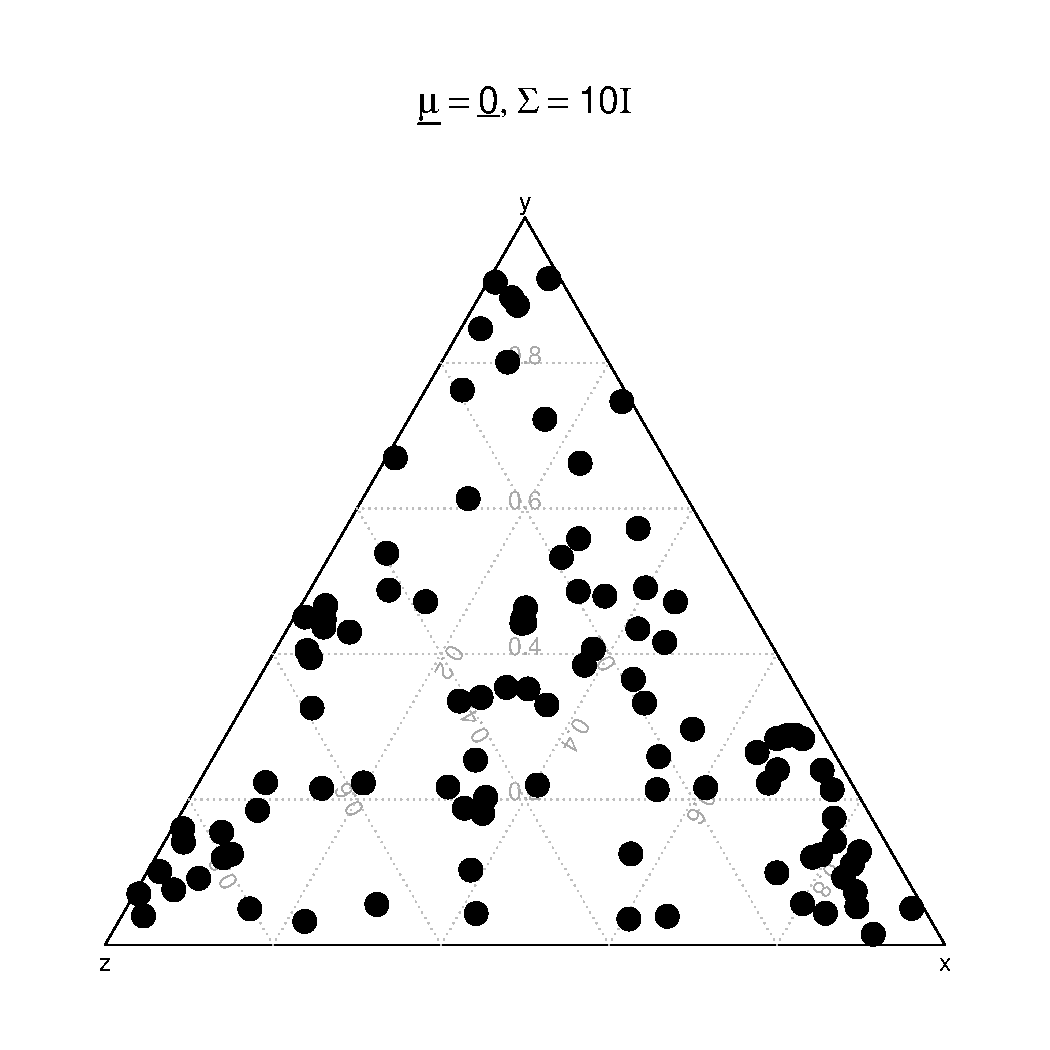
\includegraphics[scale=0.25]{figures/sigma3_3_bw.pdf}} \\
%  \num\putindeepbox[2pt]{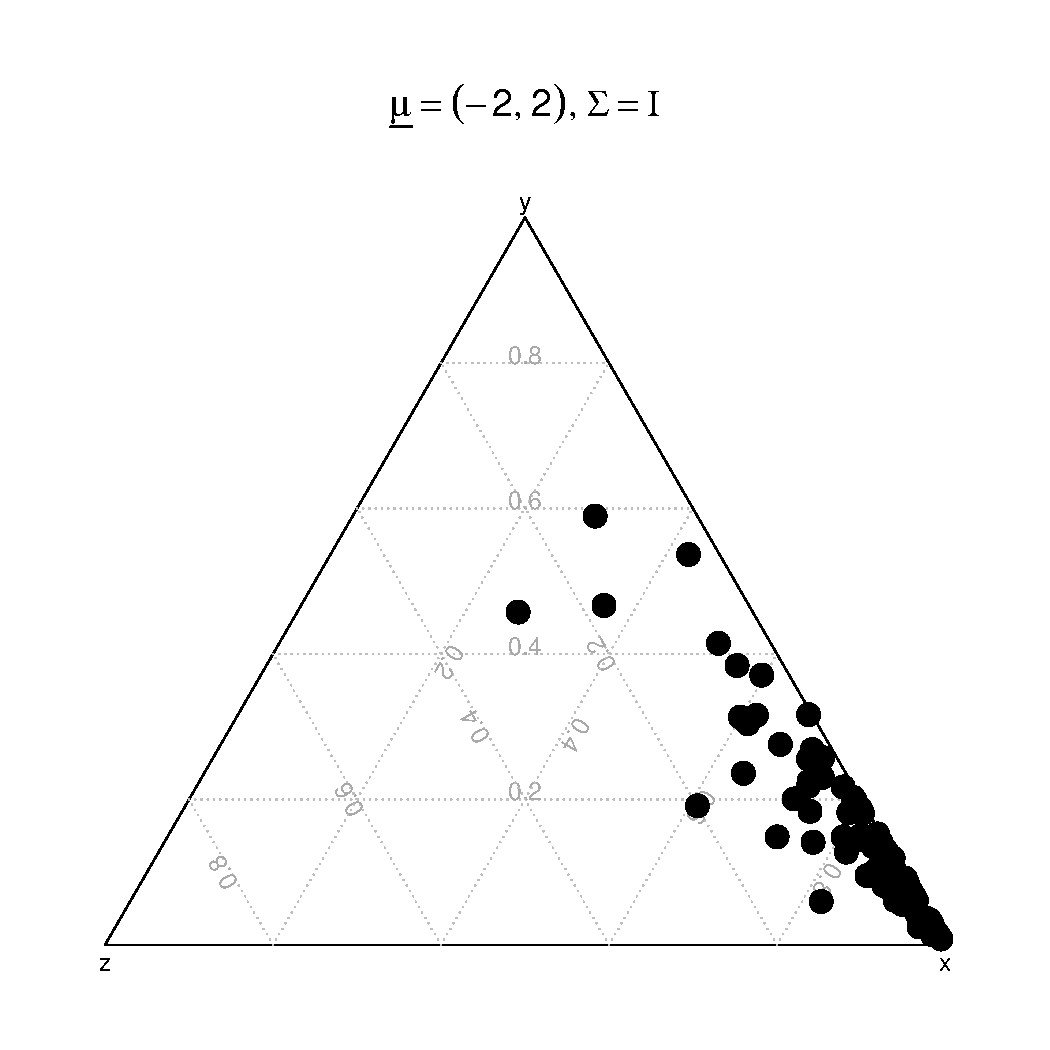
\includegraphics[scale=0.25]{figures/mu2_0_bw.pdf}}
%    & \num\putindeepbox[2pt]{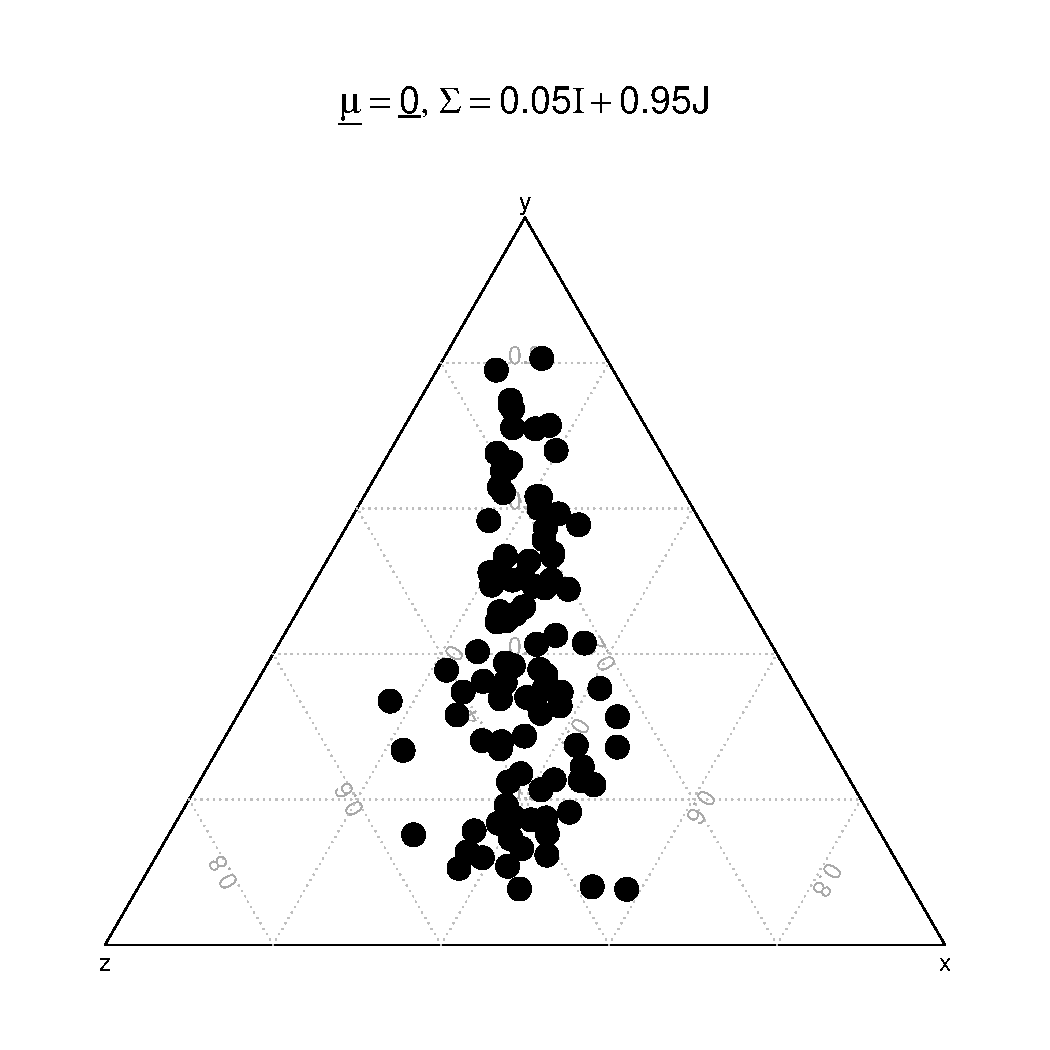
\includegraphics[scale=0.25]{figures/sigma1_9_9_1_bw.pdf}} \\
\end{tabular}
\caption{write the caption here.}
\label{fig:interaction_trees}
\end{center}
\end{figure} 

We ran the ALoVaS and DiVaS algorithms for $11,000$ samples discarding the first $1000$ as a burn-in sample. Convergence statistics were calculated using the coda package in R with \textbf{??} statistics indicating a minimal sample size of 3764 and 3271 for the ALoVaS and DiVaS chains respectively. The trees with the largest integrated likelihood for the two chains are presented in Figure \ref{fig:chain_max_interaction_tree}.  

\begin{figure}
\begin{center} 
\begin{tabular}{cc}
%  \num\putindeepbox[2pt]{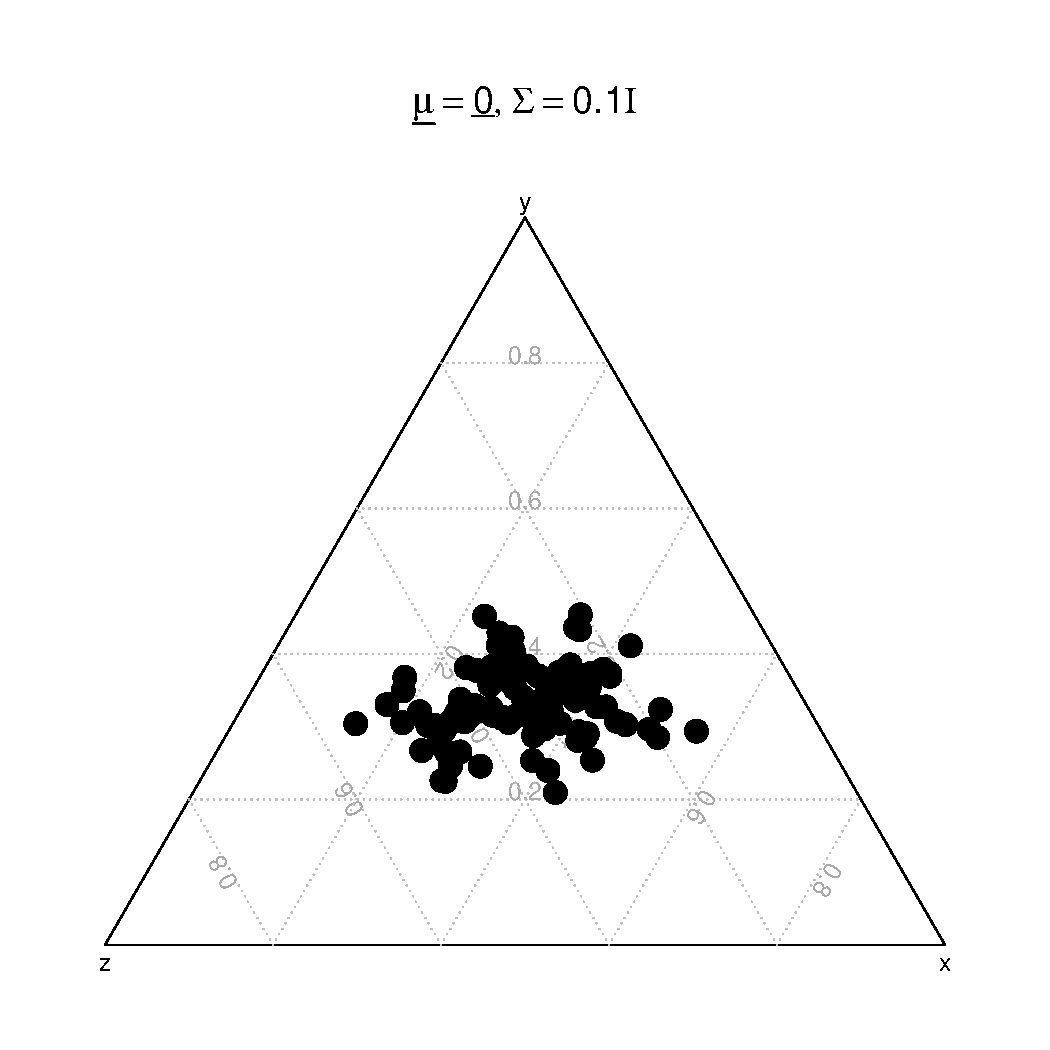
\includegraphics[scale=0.25]{figures/mu0_0_bw.pdf}}
%    & \num\putindeepbox[2pt]{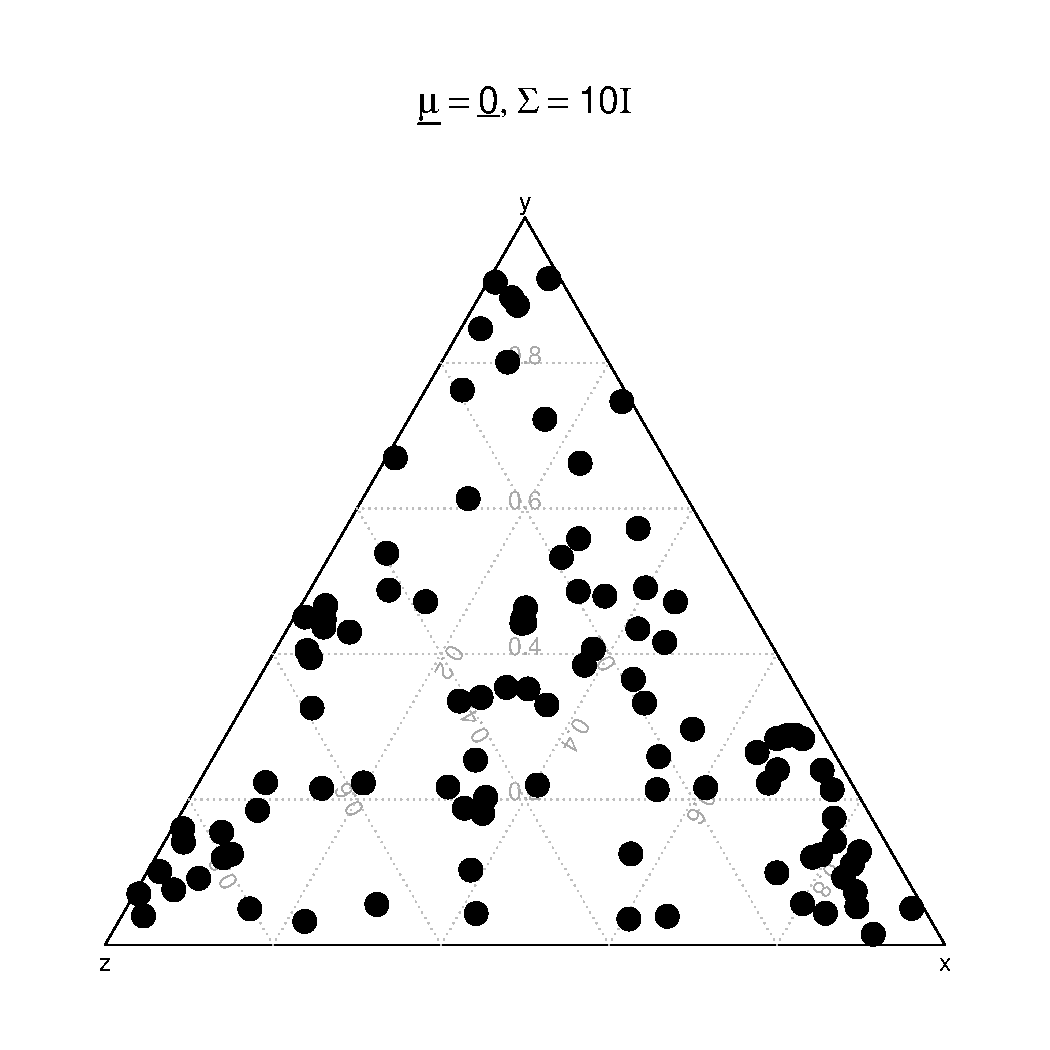
\includegraphics[scale=0.25]{figures/sigma3_3_bw.pdf}} \\
%  \num\putindeepbox[2pt]{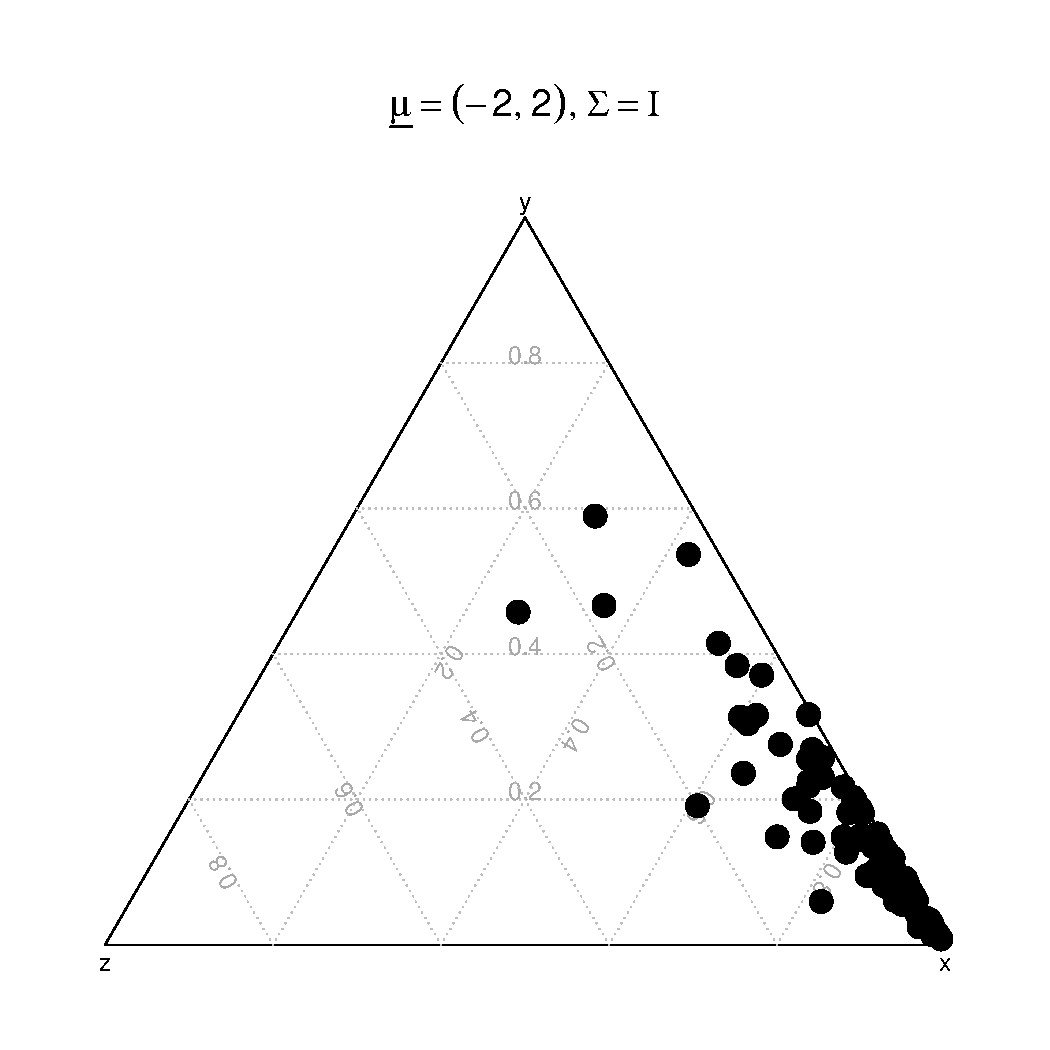
\includegraphics[scale=0.25]{figures/mu2_0_bw.pdf}}
%    & \num\putindeepbox[2pt]{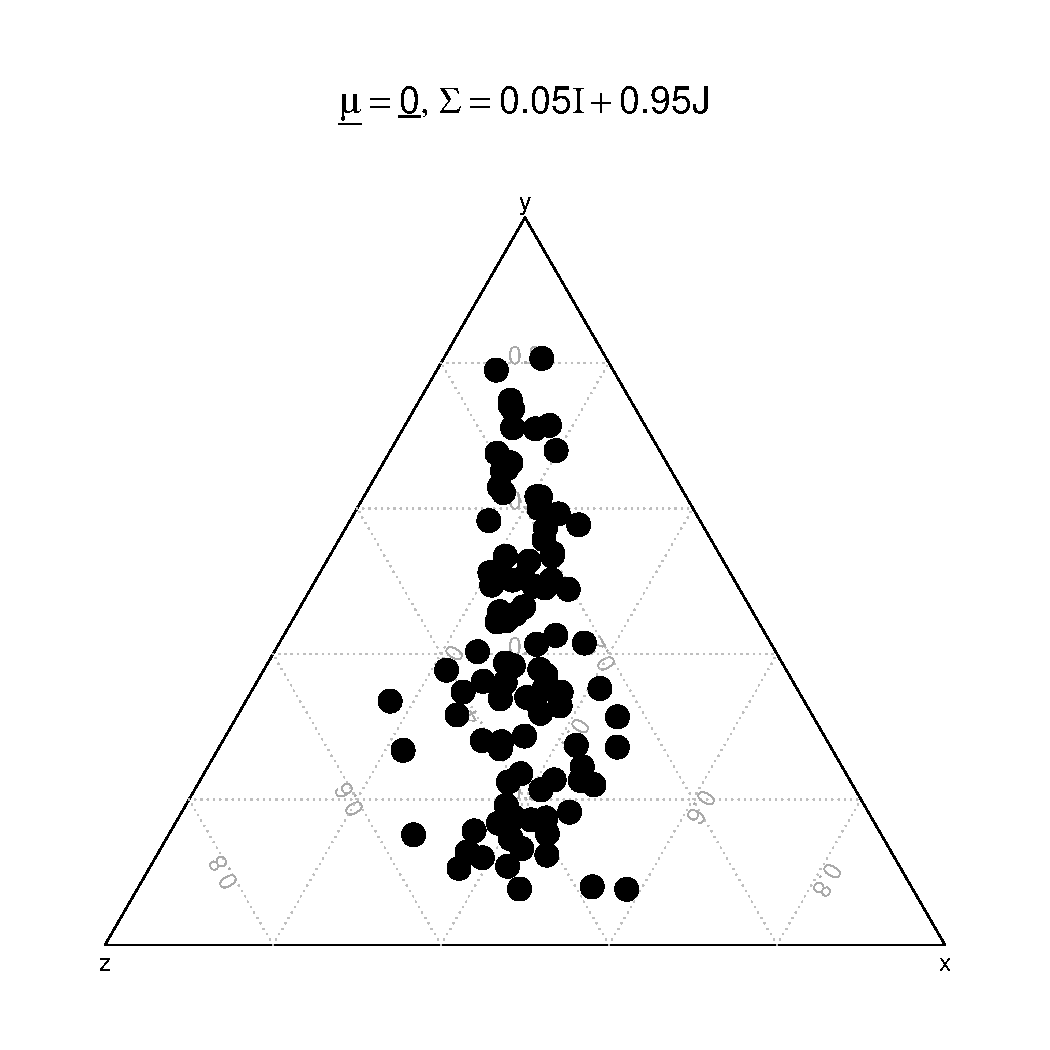
\includegraphics[scale=0.25]{figures/sigma1_9_9_1_bw.pdf}} \\
\end{tabular}
\caption{write the caption here.}
\label{fig:chain_max_interaction_tree}
\end{center}
\end{figure} 

\subsection{Practical differences and a simulation study}

While the theoretical differences are important to academics and applied researchers who want to understand the limitations of a specific method, the questions most applied researchers tend to have are more practical in nature. We address the practical questions in this section. 

Practically speaking the ALoVaS and the DiVaS methods are different in terms of how you can think about selecting a variable to split on, or to remove, from the current decision tree. While the DiVaS method allows us to \emph{quantify} these different scenarios it does not allow us to think about these values in a manner we are familiar with, whereas the ALoVaS method allows us a nice, linear framework to understand these differences. The primary difficulty lies in no standard, intuitive, basis to describe the simplex. Aitchison \ref{} discussed several bases, none of which are intuitive, whereas Euclidean geometric space is intuitive, ubiquitous, and all statisticians can be expected to have experience with the Euclidean space.   

Apart from this there are other more practical differences between the DiVaS and ALoVaS methods. For example, the ALoVaS method takes much longer to simulate. This additional simulation time should be no surprise given the additional number of parameters to simulate in the ALoVaS model relative to the DiVaS model. In the ALoVaS model we typically have means, variances, and covariances to simulate one for each covariate and then global ones as well. This difference is one reason why the sampling takes longer. A second reason comes from the methods used to simulate the parameters from the DiVaS and ALoVaS methods. While the Dirichlet density is complicated because of the relationship with the gamma density there are highly optimized sampling codes for the Dirichlet density which have been used in production since at least the early 1990s and can be considered stable and highly optimized. In contrast to this, the lasso ALoVaS model requires sampling from a generalized inverse Gaussian density which is complicated to sample from. While several algorithms exist it is unclear what is the optimal algorithm for a given scenario. Nevertheless, there are well known accept-reject methods to sample the generalized inverse Gaussian density but they require more work to draw a sample (1.58 samples on average)  than more straightforward sampling methods like the polar method most commonly used to sample the Dirichlet density. In addition the sampling for the generalized inverse Gaussian density typically requires evaluating special functions like the Bessel function adding to the computational time at each iteration. 

A further practical difficulty that distinguishes the two methods is the correlations between the covariate selection probabilities. Recall the DiVaS method requires that the correlations between covariate selection probabilities are negative \emph{a priori}. Whereas the ALoVaS method allows the correlation between any two covariate selection probabilities to be any value in the range $[-1,1]$, the typical area of support for a correlation. The practical difficulty then with the DiVaS method is that it is impossible to know whether the covariate selection probabilities are negative, positive, or zero. Thus, using the DiVaS method seems to be asking for model misspecification errors. Moreover, if the model is linear with significant interactions, as shown earlier in this chapter and we estimate the response with a decision tree, then we will have positive covariate selection probabilities. 
In fact any model having a curvature in two or more of the covariates implies that when we build a decision tree we will have a positive covariate selection probability regardless of whether the generative model is linear or not, curvature of the model indicates positive covariate selection probabilities. 

A reasonable question the reader may ask now is: if positive correlations of the covariate selection probabilities are a result of curvature when do negative correlation occur? In this case we would need covariates to split in the decision tree but we would want to select either $x_1$ or $x_2$ but not both. As one simple example this might occur if the generative model was 

\begin{equation}
y_i = \beta_1x_1 + \beta_2x_2 + \epsilon_i
\end{equation}
 for $i=1, \dots, n$ and the two covariates $x_1$ and $x_2$ were such that $Corr(x_1, x_2) \neq 0$. In this case we see that knowledge of one covariate indicates knowledge of the other covariate as well, if not exact then at least approximately.   In this case we would need the generative model to be linear because the correlation  is a bilinear operator. In this case, we could choose to split on $x_1<c$ for some constant $c$ or we could choose to split on $x_2 < c^\prime$ for some value $c^\prime$ because the two covariates are correlated, knowledge of one implies approximate knowledge of the other and therefore we would only need to split on one and not the other covariate. Thus in this case if covariate $x_1$ is split on for example, the prevalence of a split on covariate $x_2$ would not only be unlikely, but it would also be unnecessary, provided  $|Corr(x_1, x_2)|$ was large enough. 
 
\subsection{Conclusions and Recommendations}

The similarities and the differences between the ALoVaS and DiVaS methods having been pointed out, we now turn to the conclusions and recommendations we have for the use of the two methods. 

While the DiVaS method is a theoretically sound method, several theoretical and practical difficulties arise when trying to implement the method. In contrast the ALoVaS method has few theoretical difficulties and the practical difficulties are primarily in terms of time to simulate which will typically not be an issue for scientific problems and most problems with no dynamic, or time varying component. Therefore, problems involving decision trees where the data occur on a timescale less than 1 day and especially less than an hour will likely not find use in the DiVaS and ALoVaS methods. Those needing these short timeframe models are likely to find some use in the time varying decision trees proposed by Gramacy, Taddy, and Polson \cite{taddy2011dynamic}. Moreover, the approach of the DiVaS method is more of an ad-hoc method lacking a unifying idea whereas the ALoVaS method has one underlying concept, the ALT to transform from a linear scale to a probability scale. 

The conclusion then seems straightforward if one is to choose between the DiVaS and the ALoVaS methods one would choose the ALoVaS method because of the  theoretical soundness, the conceptual link with linear methods, and for the ease of implementation. The key drawbacks being the run-time of the algorithm and the need to choose one of the regularization techniques discussed in this text or one of the plethora of other regularization techniques available in the statistics literature. However as indicated in Section \ref{}  the choice of which ALoVaS method to use is dependent largely on the underlying DGP, the knowledge of which would preclude the model fitting exercise. Also, our simulation studies in Section \ref{} largely indicate that within a given sparsity level, the  choice of which type of ALoVaS method is largely irrelevant. To reiterate, the ALoVaS method, of any type is to be preferred to the DiVaS method. 

